\documentclass{beamer}
\usepackage{graphicx}

\usepackage{amssymb} %Ajoute des symboles mathématiques comme R, Z, forall, exists, etc....
\usepackage{amsmath}
\usepackage{amsthm}

\usepackage{pgf} %permet d'introduire des images vectorielles pour les présentations 
\usepackage{tikz} %permet de créer des graphiques dans le texte 

\usepackage[french,vlined,lined,linesnumbered,boxed]{algorithm2e}

\usetheme{Frankfurt}


\title{\textbf{Présentation des différents types de parcours d'arbres en informatique}}
\author{Derrez Lorenzo}

\begin{document}

\begin{frame}{\textbf{ATTENTION :}}
    \begin{center}
        \qquad -- Ceci est une présentation exhaustive afin de m'entraîner à utiliser le module "Beamer" et "Tikz".
    \end{center}
\end{frame}

\begin{frame}
    \maketitle
    \centering
\end{frame}

\begin{frame}{\textbf{Sommaire :}}
    \begin{enumerate}
        \item Parcours en largeur
        \item Parcours en profondeur
        \begin{itemize}
            \item Parcours en profondeur infixe
            \item Parcours en profondeur préfixe
            \item Parcours en profondeur suffixe
        \end{itemize}
    \end{enumerate}
\end{frame}

\begin{frame}{\textbf{Parcours en largeur}}
    \begin{block}{Introduction}
        \begin{algorithm}[H]
            \footnotesize
            \caption{Parcours en largeur}
            \Donnees{racine}
            \If{racine est vide}{
                \Return []
            }
            \Else{
                F $\leftarrow$ creer\_file()
                \\
                enfiler(racine, F)
                \\
                \Tq{F n'est pas vide}{
                    noeud $\leftarrow$ defiler(F)
                    \\
                    traiter(noeud)
                    \\
                    \If{noeud.gauche != nul}{
                        enfiler(noeud.gauche)
                    }
                    \If{noeud.droite != nul}{
                        enfiler(noeud.droite)
                    }
                }
            }
        \end{algorithm}
    \end{block}
\end{frame}

\begin{frame}{\textbf{Parcours en largeur}}
    \begin{block}{Illustrations}
        \centering
        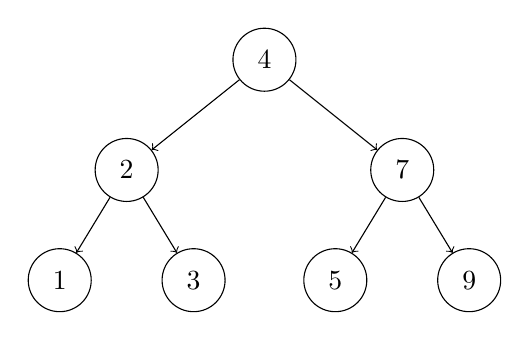
\begin{tikzpicture}[
            nodes={draw, circle, minimum size=8mm},
            level 1/.style={sibling distance=35mm},
            level 2/.style={sibling distance=17mm},
            level distance=14mm,
            ->
        ]
            \node {4}
                child { node {2}
                    child { node {1} }
                    child { node {3} }
                }
                child { node {7}
                    child { node {5} }
                    child { node {9} }
                };
        \end{tikzpicture}
    \end{block}
\end{frame}
\end{document}